\documentclass[12pt,a4paper]{article}

\usepackage{iftex}
\ifPDFTeX
    \usepackage[T2A]{fontenc}
    \usepackage[utf8]{inputenc}
    \usepackage[russian]{babel}
\else
    \usepackage{fontspec}
    \usepackage[russian]{babel}
    \defaultfontfeatures{Ligatures=TeX}
    \setmainfont{Times New Roman}
    \setsansfont{Arial}
    \setmonofont{Consolas}
\fi
\usepackage{amsmath}
\usepackage{booktabs}
\usepackage{geometry}
\usepackage{graphicx}
\usepackage{hyperref}
\usepackage{tabularx}
\usepackage{xcolor}
\usepackage{float}
\usepackage{enumitem}

\geometry{margin=2.2cm}
\graphicspath{{report_assets/}}
\hypersetup{
    colorlinks=true,
    linkcolor=black,
    urlcolor=blue,
    citecolor=black
}

\title{Отчет по лабораторной работе №2\\Обработка изображений фишек игрового набора Тантрикс}
\author{Подъяблонский Егор Петрович, 317 группа, ММП ВМК МГУ}
\date{2026}

\begin{document}

\begin{center}
    {\LARGE \textbf{Отчет о лабораторной работе №2}\par}
    \vspace{0.3cm}
    {\Large \textbf{«Обработка изображений фишек игрового набора Тантрикс»}\par}
    \vspace{0.5cm}
    {\large Подъяблонский Егор Петрович, 317 группа, ММП ВМК МГУ\par}
\end{center}
\vspace{1cm}

\tableofcontents
\newpage

\section{Постановка задачи}
Тема лабораторной работы --- изучение и освоение методов обработки и сегментации изображений. Требуется разработать программу для анализа изображений фишек игрового набора Тантрикс. На вход подается изображение в формате BMP, на выходе программа должна выдавать описание состава и расположения фишек на изображении.

По условию задания программа должна обеспечивать:
\begin{itemize}[leftmargin=1.2cm]
    \item ввод и отображение изображений в формате BMP;
    \item сегментацию изображений на основе точечных и пространственных преобразований;
    \item генерацию признаковых описаний фишек на изображении;
    \item классификацию отдельных фишек и их последовательностей.
\end{itemize}

Задание разбито на три уровня сложности. В данной работе реализованы задачи всех трех уровней:
\begin{enumerate}[leftmargin=1.2cm]
    \item \textbf{Beginner, задача 1:} определить количество фишек на изображении типа \texttt{Group\_*.bmp}.
    \item \textbf{Beginner, задача 2:} определить тип и цвет линий на одной фишке из файла типа \texttt{Single\_*.bmp}. Возможные типы линий: короткая дуга большой кривизны, длинная дуга малой кривизны и прямолинейный сегмент.
    \item \textbf{Intermediate, задача 3:} определить номер отдельной фишки из файла типа \texttt{Single\_*.bmp}.
    \item \textbf{Intermediate, задача 4:} определить расположение и номера всех фишек в кадре для файла типа \texttt{Group\_*.bmp}.
    \item \textbf{Expert, задача 5:} определить последовательность обхода фишек в мозаике вдоль замкнутого маршрута для файла типа \texttt{Path\_*.bmp}.
\end{enumerate}

\section{Описание данных}
Игровой набор Тантрикс состоит из десяти фишек. Каждая фишка представляет собой правильный шестиугольник черного цвета. На фишке изображены сегменты трех линий: синей, красной и желтой. Линия каждого цвета соединяет две стороны шестиугольника и может быть короткой дугой, длинной дугой или прямолинейным сегментом.

К заданию прилагаются изображения разной сложности:
\begin{itemize}[leftmargin=1.2cm]
    \item \texttt{Single\_*.bmp} --- изображения одной фишки;
    \item \texttt{Group\_*.bmp} --- изображения нескольких несоприкасающихся фишек, расположенных произвольно;
    \item \texttt{Path\_*.bmp} --- мозаики из соприкасающихся фишек, в которых нужно найти замкнутый маршрут.
\end{itemize}

В работе использовались тестовые изображения из папки \texttt{Образцы}: четыре изображения \texttt{Single}, три изображения \texttt{Group} и три изображения \texttt{Path}. Для демонстрации работы программы в отчет включены примеры обработки одиночной фишки, группы фишек и мозаики.

Основные особенности данных:
\begin{itemize}[leftmargin=1.2cm]
    \item фон изображения светлый, а сами фишки темные;
    \item фишки могут быть повернуты, смещены и сняты с небольшой перспективной деформацией;
    \item цветные линии могут пересекаться, причем одна из линий визуально разрывается в точке пересечения;
    \item в изображениях \texttt{Path} соседние фишки соприкасаются гранями, поэтому обычное выделение связных компонент не разделяет их на отдельные объекты.
\end{itemize}

\section{Описание метода решения}
\subsection{Общий конвейер обработки}
Решение строится как последовательный конвейер компьютерного зрения:
\begin{enumerate}[leftmargin=1.2cm]
    \item чтение изображения и приведение его к единому цветовому представлению;
    \item сегментация темных шестиугольных объектов на светлом фоне;
    \item нормализация каждой найденной фишки к каноническому шестиугольнику;
    \item выделение цветных линий и построение признакового описания;
    \item классификация линий и номера фишки;
    \item для мозаик \texttt{Path} построение графа касаний и поиск замкнутого маршрута.
\end{enumerate}

На практике конвейер разделен на два понятных этапа: цветовая обработка быстро отделяет фон, темные фишки и цветные линии, а геометрическая обработка уточняет форму объектов, закрывает разрывы в масках и приводит каждую фишку к общей системе координат.

\subsection{Сегментация фишек}
Для изображений \texttt{Single} и \texttt{Group} используется классическая сегментация темных объектов на светлом фоне. Изображение переводится в цветовые пространства RGB, HSV и LAB, после чего фон оценивается по граничным областям кадра. Далее строится бинарная маска темных объектов, очищается морфологическими операциями и разбивается на связные компоненты. Компоненты малой площади отбрасываются как шум.

Так как фишки являются правильными шестиугольниками, итоговая маска каждой компоненты дополнительно регуляризуется: по контуру строится выпуклая оболочка, оцениваются углы и центр объекта, а затем область приводится к шестиугольной форме. Это уменьшает влияние бликов, цветных линий и небольших дырок внутри маски.

Для изображений \texttt{Path} используется отдельная ветка. Сначала выделяется общая маска всей мозаики, поскольку соприкасающиеся фишки образуют одну связную область. Затем общая область делится на отдельные шестиугольные ячейки с учетом ожидаемого количества фишек и их регулярной формы. После разделения каждая ячейка проходит ту же нормализацию, что и обычная фишка.

\subsection{Нормализация фишки}
Для каждой найденной фишки вычисляется преобразование в канонический вид. На основе маски определяется шестиугольный контур, после чего строится гомография из вершин найденного шестиугольника в фиксированный правильный шестиугольник размера $220 \times 220$ пикселей. В нормализованном изображении вершина фишки расположена снизу, а грани нумеруются снизу по часовой стрелке.

Нормализация решает две задачи. Во-первых, она устраняет поворот, масштаб и перспективные искажения. Во-вторых, она позволяет описывать линии на разных фишках в единой системе координат через номера граней, которые соединяет линия.

\subsection{Построение признакового описания}
Для каждой нормализованной фишки строятся три цветовые маски: красная, желтая и синяя. Маски выделяются по эвристическим порогам в цветовых пространствах RGB, HSV и LAB. После пороговой фильтрации применяются морфологическое закрытие, удаление мелких компонент и ограничение области поиска внутренней частью фишки.

Полученное признаковое описание каждой цветной линии содержит:
\begin{itemize}[leftmargin=1.2cm]
    \item цвет линии;
    \item пару граней шестиугольника, к которым линия подходит;
    \item тип линии: короткая дуга, длинная дуга или прямолинейный сегмент.
\end{itemize}

При пересечении линий один цветной сегмент может быть разорван на две компоненты. Поэтому при анализе учитываются не только отдельные связные компоненты маски, но и их совместное расположение относительно граней фишки.

\subsection{Классификация линий и фишек}
Тип линии определяется по взаимному расположению двух граней, которые она соединяет:
\begin{itemize}[leftmargin=1.2cm]
    \item соседние грани соответствуют короткой дуге большой кривизны;
    \item грани через одну соответствуют длинной дуге малой кривизны;
    \item противоположные грани соответствуют прямолинейному сегменту.
\end{itemize}

Номер фишки определяется сравнением полученного признакового описания с эталонным описанием десяти фишек набора Тантрикс. Для каждой фишки известны цвета, типы линий и пары соединяемых граней. Выбирается номер с минимальной стоимостью расхождения между найденными и эталонными признаками. Для групповых изображений дополнительно используется требование, что в одном наборе не должно быть повторов номеров фишек.

\subsection{Построение маршрута в мозаике}
Для задачи уровня Expert после распознавания фишек строится граф касаний. Вершинами графа являются найденные фишки, а ребра соответствуют соприкосновению двух фишек по граням. Для каждой пары соседних фишек определяется номер контактной грани у каждой из них.

Поиск маршрута выполняется перебором допустимых стартов:
\begin{enumerate}[leftmargin=1.2cm]
    \item выбирается самая нижняя фишка мозаики;
    \item среди ее контактных граней ищется пара, соединенная линией одного цвета;
    \item выбирается направление обхода, после чего переход выполняется через соседнюю фишку по контактной грани;
    \item на новой фишке маршрут продолжается по линии того же цвета от входной грани к выходной;
    \item если обход возвращается в стартовую фишку и образует замкнутую последовательность, маршрут считается найденным.
\end{enumerate}

Если для выбранной пары граней маршрут не замыкается, проверяется следующая допустимая пара. Число фишек невелико, поэтому такой перебор работает быстро и напрямую использует геометрию касаний фишек.

\section{Описание программной реализации}
Программа реализована на языке Python. Для обработки изображений используются OpenCV и NumPy, для интерфейса --- Tkinter, для вывода изображений в интерфейсе --- Pillow.

Код разделен на несколько модулей:
\begin{itemize}[leftmargin=1.2cm]
    \item \texttt{app.py} --- графический интерфейс: выбор BMP-файла, отображение исходного изображения, маски фишек, нормализованных фишек и результатов распознавания;
    \item \texttt{debug\_pipeline.py} --- основной конвейер обработки одного изображения;
    \item \texttt{image\_io.py} --- безопасное чтение изображений, в том числе из путей с кириллическими символами;
    \item \texttt{segmentation\_tiles.py} --- построение масок фишек для изображений \texttt{Single}, \texttt{Group} и \texttt{Path};
    \item \texttt{tile\_normalization.py} --- приведение фишки к каноническому шестиугольнику;
    \item \texttt{tile\_line\_masks.py} --- выделение красной, желтой и синей линий;
    \item \texttt{line\_classification.py} --- определение типа линии по соединяемым граням;
    \item \texttt{tile\_identification.py} --- сопоставление признаков с эталонными описаниями десяти фишек;
    \item \texttt{route\_analysis.py} --- построение графа касаний и поиск замкнутого маршрута.
\end{itemize}

Графический интерфейс используется не только для демонстрации результата, но и для отладки промежуточных этапов. Пользователь может увидеть исходное изображение с подписанными номерами фишек, общую маску найденных фишек, нормализованные фишки с наложенными цветовыми масками линий и итоговую строку маршрута для мозаик.

\section{Эксперименты}
\subsection{Иллюстрации работы программы}
На рисунках~\ref{fig:single1}, \ref{fig:group5}, \ref{fig:path10} показаны результаты работы программы на трех типах изображений из задания.

\begin{figure}[H]
    \centering
    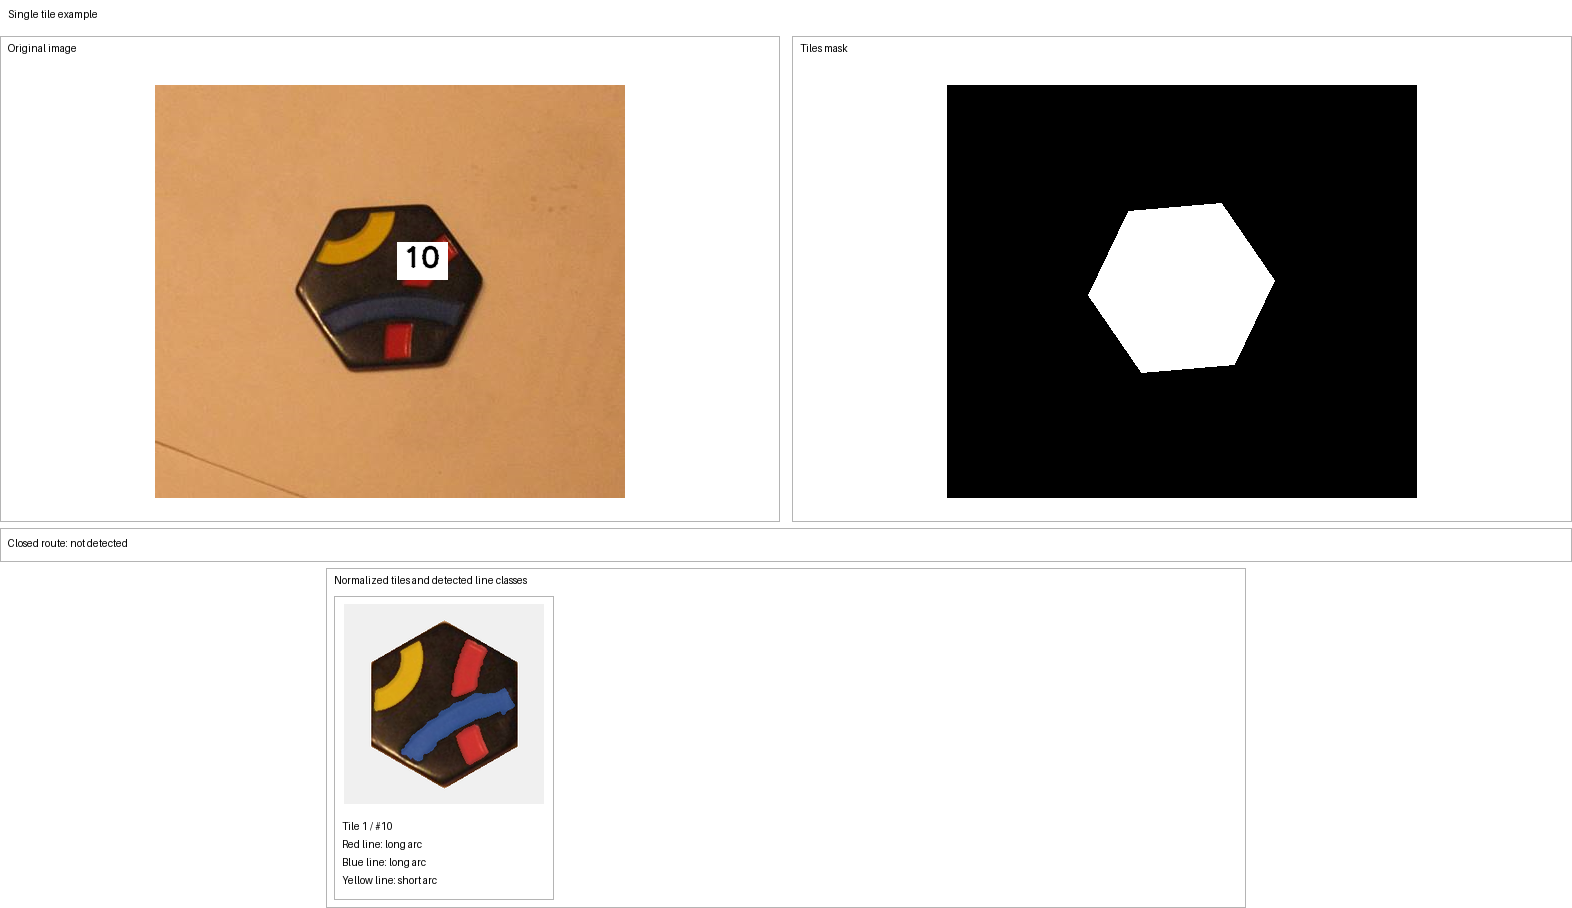
\includegraphics[width=\textwidth]{single1_pipeline.png}
    \caption{Обработка изображения одной фишки \texttt{Single\_1.bmp}: исходное изображение, маска и нормализованная фишка с линиями}
    \label{fig:single1}
\end{figure}

\begin{figure}[H]
    \centering
    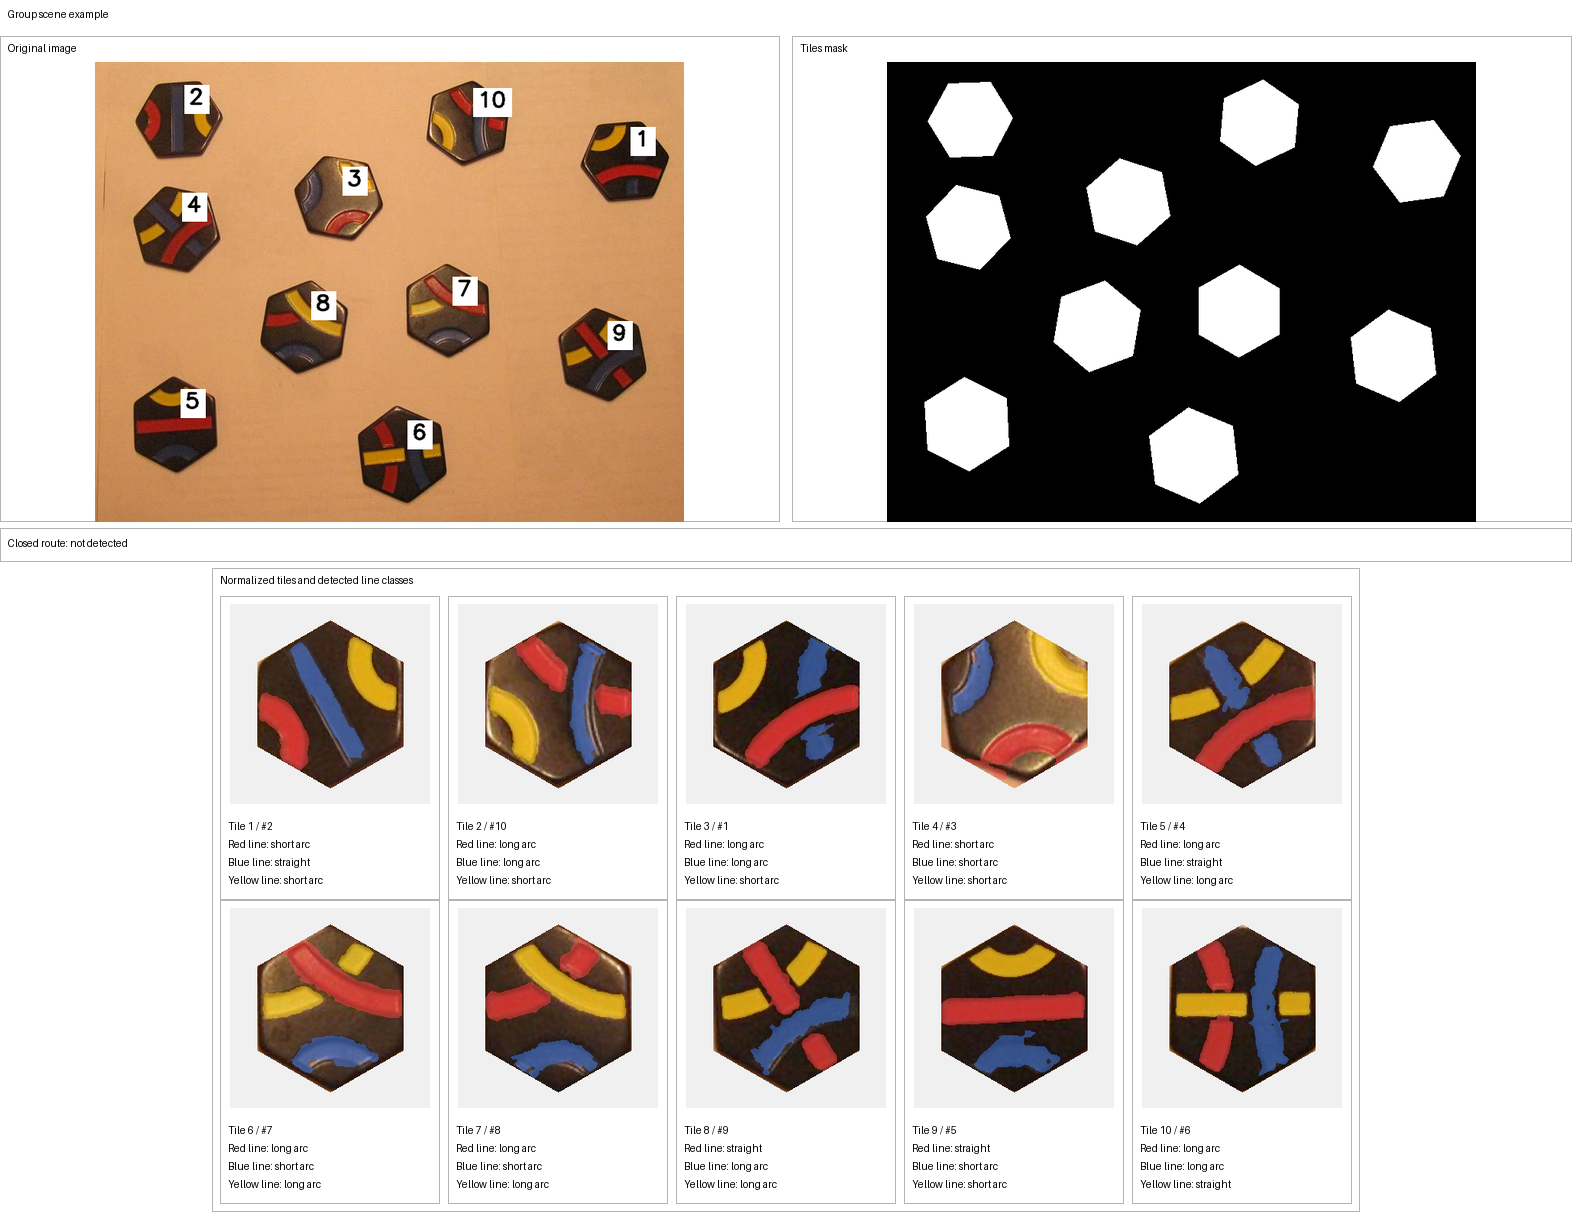
\includegraphics[width=\textwidth]{group5_pipeline.png}
    \caption{Обработка изображения группы фишек \texttt{Group\_5.bmp}: определение количества, расположения и номеров фишек}
    \label{fig:group5}
\end{figure}

\begin{figure}[H]
    \centering
    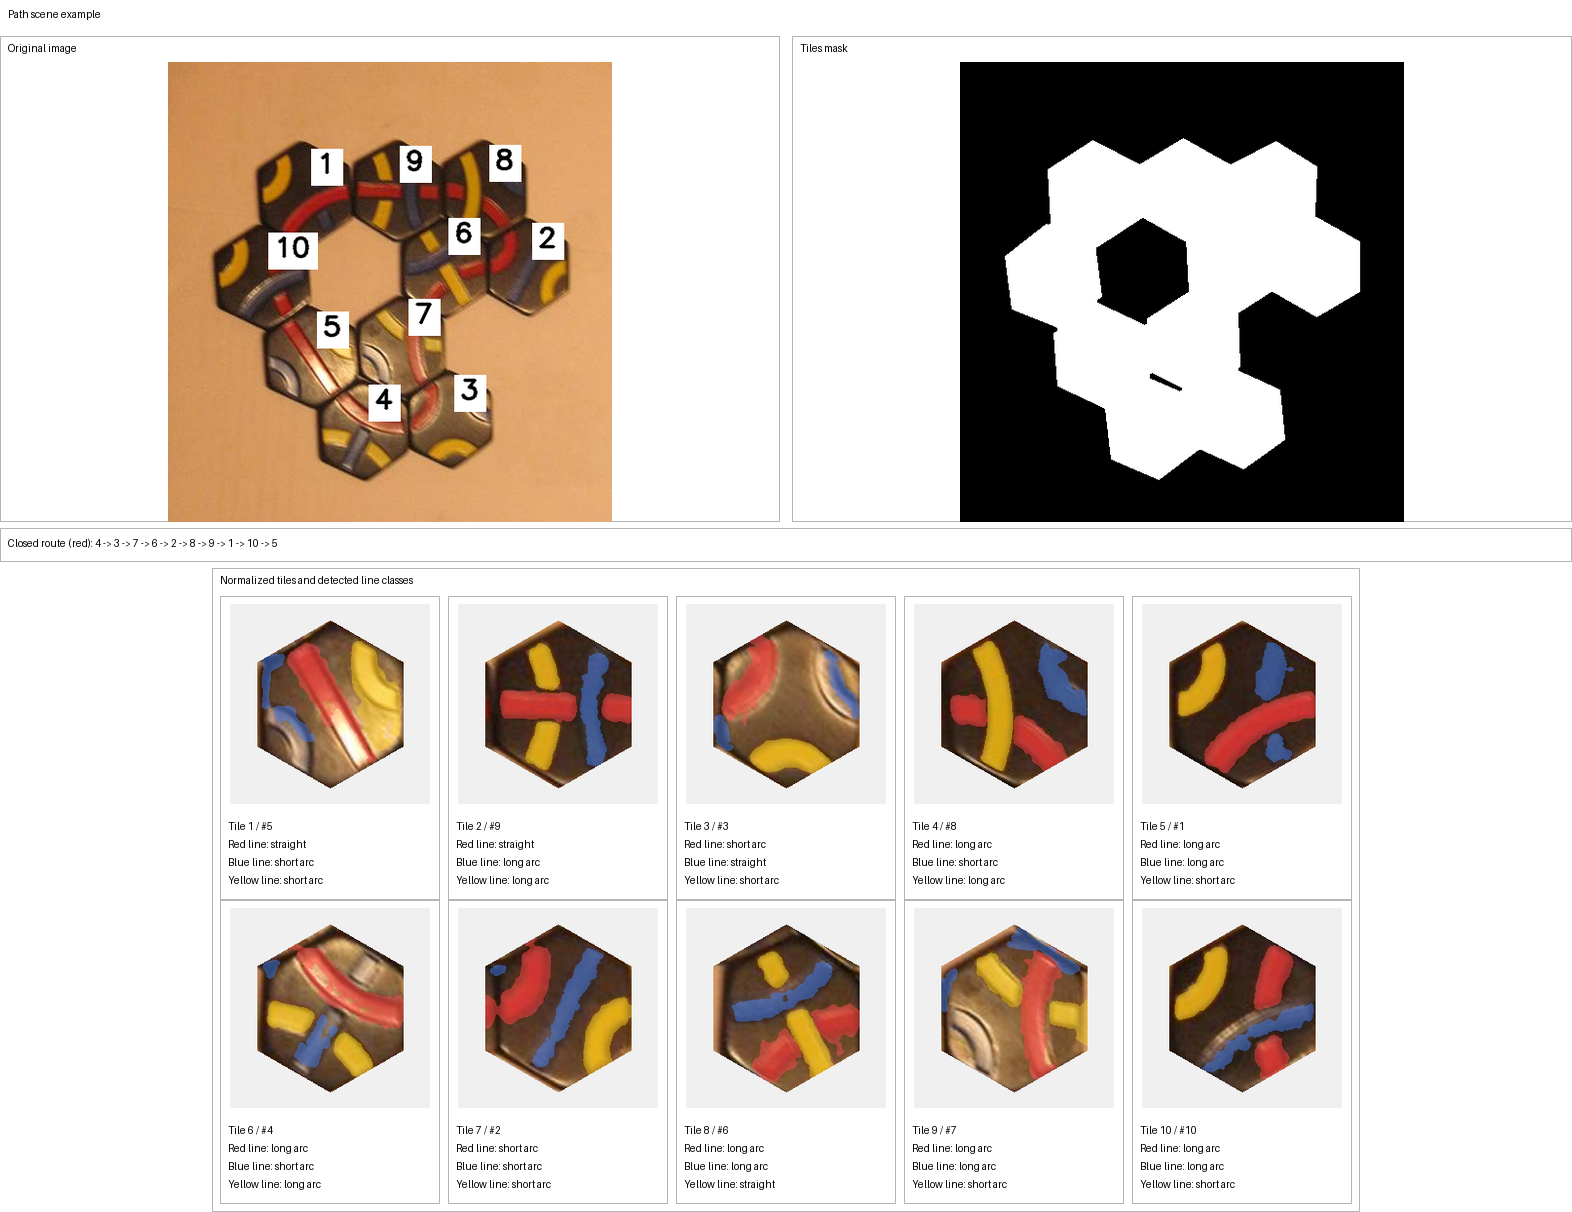
\includegraphics[width=\textwidth]{path10_pipeline.png}
    \caption{Обработка мозаики \texttt{Path\_10\_1.bmp}: сегментация соприкасающихся фишек и поиск замкнутого маршрута}
    \label{fig:path10}
\end{figure}

\subsection{Результаты задач Beginner и Intermediate}
В таблице~\ref{tab:results-single} приведены результаты для одиночных фишек. Эти эксперименты проверяют задачу 2 уровня Beginner и задачу 3 уровня Intermediate.

\begin{table}[H]
    \centering
    \small
    \caption{Классификация линий и номеров фишек на изображениях \texttt{Single}}
    \label{tab:results-single}
    \begin{tabularx}{\textwidth}{l X c}
        \toprule
        Изображение & Распознанные линии & Номер фишки \\
        \midrule
        \texttt{Single\_1.bmp} & желтая короткая дуга, красная длинная дуга, синяя длинная дуга & 10 \\
        \texttt{Single\_2.bmp} & синяя короткая дуга, желтая длинная дуга, красная длинная дуга & 7 \\
        \texttt{Single\_3.bmp} & синяя короткая дуга, желтая короткая дуга, красная короткая дуга & 3 \\
        \texttt{Single\_4.bmp} & синяя короткая дуга, красная прямая, желтая короткая дуга & 5 \\
        \bottomrule
    \end{tabularx}
\end{table}

В таблице~\ref{tab:results-group} приведены результаты для групп фишек. Эти эксперименты проверяют задачу 1 уровня Beginner и задачу 4 уровня Intermediate.

\begin{table}[H]
    \centering
    \small
    \caption{Определение количества, расположения и номеров фишек на изображениях \texttt{Group}}
    \label{tab:results-group}
    \begin{tabularx}{\textwidth}{l c X}
        \toprule
        Изображение & Количество фишек & Распознанные номера \\
        \midrule
        \texttt{Group\_1.bmp} & 3 & [8, 2, 10] \\
        \texttt{Group\_3.bmp} & 3 & [1, 9, 6] \\
        \texttt{Group\_5.bmp} & 10 & [2, 10, 1, 3, 4, 7, 8, 9, 5, 6] \\
        \bottomrule
    \end{tabularx}
\end{table}

\subsection{Результаты задачи Expert}
В таблице~\ref{tab:results-path} приведены результаты для мозаик. Для каждой мозаики программа определяет номера фишек и последовательность обхода вдоль найденного замкнутого маршрута.

\begin{table}[H]
    \centering
    \small
    \caption{Поиск замкнутого маршрута на изображениях \texttt{Path}}
    \label{tab:results-path}
    \begin{tabularx}{\textwidth}{l X X}
        \toprule
        Изображение & Распознанные номера фишек & Найденный маршрут \\
        \midrule
        \texttt{Path\_4.bmp} & [8, 5, 7, 3] & 3 $\rightarrow$ 7 $\rightarrow$ 5 $\rightarrow$ 8 \\
        \texttt{Path\_7\_1.bmp} & [9, 6, 7, 5, 1, 8, 4] & 5 $\rightarrow$ 9 $\rightarrow$ 7 $\rightarrow$ 6 $\rightarrow$ 1 $\rightarrow$ 4 $\rightarrow$ 8 \\
        \texttt{Path\_10\_1.bmp} & [5, 9, 3, 8, 1, 4, 2, 6, 7, 10] & 4 $\rightarrow$ 3 $\rightarrow$ 7 $\rightarrow$ 6 $\rightarrow$ 2 $\rightarrow$ 8 $\rightarrow$ 9 $\rightarrow$ 1 $\rightarrow$ 10 $\rightarrow$ 5 \\
        \bottomrule
    \end{tabularx}
\end{table}

На использованном тестовом наборе программа корректно решает все заявленные задачи: считает фишки на групповых изображениях, строит признаки линий на одиночных фишках, определяет номера фишек, подписывает их расположение в кадре и находит маршрут в мозаиках.

Наиболее сложным примером оказалась мозаика \texttt{Path\_10\_1.bmp}. По сравнению с остальными изображениями она имеет менее стабильное качество: хуже различаются границы соседних фишек и местами слабее выражены цветные линии. Поэтому именно этот файл стал основной проверкой устойчивости сегментации соприкасающихся шестиугольников и последующего построения маршрута.

\section{Выводы}
В ходе работы была разработана программа для обработки изображений фишек игрового набора Тантрикс. Реализация покрывает задачи уровней Beginner, Intermediate и Expert из постановки: от подсчета фишек и классификации цветных линий до определения номеров фишек и построения последовательности обхода в мозаике.

Основной результат работы --- конвейер обработки изображений, который объединяет цветовую сегментацию, морфологическую обработку, геометрическую нормализацию шестиугольников, построение признаковых описаний и графовый анализ касаний. Графический интерфейс позволяет наглядно проверять промежуточные маски и итоговую классификацию, что упрощает демонстрацию и отладку решения.

\end{document}
